\documentclass[11pt]{amsart}
\usepackage[margin=1.1in]{geometry}
\usepackage{amssymb,booktabs,hyperref}
\hypersetup{colorlinks=true,linkcolor=blue,citecolor=blue,urlcolor=blue}

\newtheorem{theorem}{Theorem}[section]
\newtheorem{proposition}[theorem]{Proposition}
\newtheorem{lemma}[theorem]{Lemma}
\newtheorem{corollary}[theorem]{Corollary}
\theoremstyle{definition}
\newtheorem{definition}[theorem]{Definition}
\newtheorem{remark}[theorem]{Remark}
\newtheorem{question}[theorem]{Question}

\newcommand{\bal}[1]{\langle #1\rangle}
\newcommand{\B}{\mathcal{B}}
\newcommand{\Z}{\mathbb{Z}}
\newcommand{\N}{\mathbb{N}}

\title[Quotients of zero-free balanced ternary numbers]{Infinitely many integers that are not quotients of\\ zero-free balanced ternary numbers}
\author{Vamshi Jandhyala}
\date{Preprint, version 1, 8 October 2026. Not peer reviewed.}
\subjclass[2020]{11A63, 11B85, 68V15}
\keywords{balanced ternary, digit restrictions, quotient sets, finite automata, formal verification}

\usepackage{graphicx}
\begin{document}

\begin{abstract}
Let $\B$ be the set of positive integers whose balanced ternary representation uses only the digits
$1$ and $-1$. Selfridge and Lacampagne asked whether every integer $n\not\equiv 0\pmod 3$ is a quotient
of two elements of $\B$. Bai, Meleshko, Riasat and Shallit found seventeen exceptions, the largest
$3649$, and remarked that there are likely infinitely many, without proof. We prove that $4\cdot 3^k+5$,
$4\cdot 3^k-5$, $8\cdot 3^k+7$ and $8\cdot 3^k+17$ lie outside $\B/\B$ for every $k\ge 5$, and
$8\cdot 3^k-7$ for every $k\ge 7$; each bound on $k$ is sharp. The proof exhibits, for each family, a
set of carries of size linear in $k$ that is closed under the carry map of multiplication by $n$ and
contains no accepting carry. For $4\cdot 3^k+5$ the argument is short enough to check by hand. The same method, applied
to one residue class of $k$ modulo $2$ or $4$ at a time, proves eight further families, among them
$5\cdot 3^k+4$ for $k\equiv 0\pmod 4$ and $5\cdot 3^k-4$ for $k\equiv 2\pmod 4$. All thirteen results
are formally verified in Lean~4. Of the $200$ exceptions below $10^8$, $75$ are covered. For the analogous problem with the digits $0$ and $1$ we confirm one
further case of the guess of Bai et al.\ that $621\cdot 3^{4k}-20$ always gives an exception.
\end{abstract}

\maketitle

\noindent\emph{Status of this preprint.} Theorems~\ref{thm:main} and~\ref{thm:classes} are formally verified in Lean~4 (Section~\ref{sec:lean}), using only Lean's standard axioms, and every number quoted in the paper is recomputed by a separate program (see \emph{Code and data}). This version has not yet been independently reviewed.

\section{Introduction}

Can every integer that is not divisible by $3$ be written as a quotient $N/m$ of two positive
integers whose balanced ternary digits are all $1$ or $-1$? For example, $8=9-1$ has a zero digit, but
$8=16/2$ with $16=27-9-3+1$ and $2=3-1$. John Selfridge and Carole Lacampagne asked this question, and
Guy records it in Section~F31 of \emph{Unsolved Problems in Number Theory} \cite[pp.~403--404]{Guy04},
noting that experiments suggested the answer yes. Bai et al.\ trace it to \S7 of the paper of Loxton and
van der Poorten on the analogous problem in base four \cite{LvdP}. Questions of this kind ask which
integers lie in the quotient set of a set defined by its digits; Rowland and Shallit place such
quotient sets in the framework of automatic sets of rational numbers and list related decision
problems among their open questions \cite{RS}.

To fix notation, every integer $x$ has a unique balanced ternary representation
$x=\sum_{j=0}^{L-1}\varepsilon_j 3^j$ with $\varepsilon_j\in\{-1,0,1\}$ and, if $x\ne 0$,
$\varepsilon_{L-1}\ne 0$. Call $x$ \emph{zero-free} if $x\ne 0$ and every $\varepsilon_j$ is nonzero, and
let
\[
\B=\{1,2,4,5,7,11,13,14,16,20,22,\dots\}
\]
be the set of positive zero-free integers. Since every element of $\B$ is prime to $3$, so is every
integer in the quotient set $\B/\B=\{N/m : N,m\in\B\}$, and the question is whether every integer
$n\equiv\pm1\pmod 3$ lies in $\B/\B$.

The answer is no. Bai, Meleshko, Riasat and Shallit \cite{BMRS} found the exceptions
\[
\begin{gathered}
247,\ 277,\ 967,\ 977,\ 1211,\ 1219,\ 1895,\ 1937,\ 1951,\\
1961,\ 2183,\ 2191,\ 2911,\ 2921,\ 3029,\ 3641,\ 3649,
\end{gathered}
\]
the first of which had also been found by Coppersmith \cite[F31]{Guy04}, and wrote: ``It seems likely
that there are infinitely many such counterexamples, but we have no proof.'' We supply a proof.

\begin{theorem}\label{thm:main}
For every $k\ge 5$, none of
\[
4\cdot 3^k+5,\qquad 4\cdot 3^k-5,\qquad 8\cdot 3^k+7,\qquad 8\cdot 3^k+17
\]
lies in $\B/\B$, and for every $k\ge 7$, $8\cdot 3^k-7$ does not lie in $\B/\B$. The bounds on $k$ are
sharp: the four numbers with $k=4$, and $8\cdot 3^6-7$, all lie in $\B/\B$.
\end{theorem}

\begin{corollary}
There are infinitely many positive integers $n\not\equiv 0\pmod 3$ with $n\notin\B/\B$.
\end{corollary}

Several further families are exceptions only along a residue class of $k$, or are proved here only
along one.

\begin{theorem}\label{thm:classes}
The following integers are not in $\B/\B$:
\begin{enumerate}
\item $8\cdot 3^k-17$ and $16\cdot 3^k+17$ for every even $k\ge 6$;
\item $10\cdot 3^k-11$, $10\cdot 3^k-19$, $20\cdot 3^k-19$ and $5\cdot 3^k-4$ for every
$k\equiv 2\pmod 4$ with $k\ge 6$;
\item $5\cdot 3^k+4$ for every $k\equiv 0\pmod 4$ with $k\ge 8$, and $40\cdot 3^k+41$ for every
$k\equiv 0\pmod 4$ with $k\ge 12$.
\end{enumerate}
Each bound is sharp within its residue class: the previous member of the class lies in $\B/\B$.
\end{theorem}

For the first five families in Theorem~\ref{thm:classes}, every exception below $10^8$ of the form
$a\cdot 3^k+b$ lies in the stated residue class, so the theorem accounts for all of them in that range.

Six of the seventeen exceptions above, namely $967$, $977$, $1951$, $1961$, $2911$ and $2921$,
belong to our families. Of the $200$ exceptions below $10^8$ (Section~\ref{sec:data}), $50$ belong to
the five families of Theorem~\ref{thm:main} and $75$ to the families of Theorems~\ref{thm:main}
and~\ref{thm:classes} together.

The method is a finite automaton argument made uniform in $k$. Multiplying a zero-free number by $n$
from the least significant digit upwards is governed by a carry, and $n\in\B/\B$ exactly when some
sequence of carries starting at $0$ ends in a carry that is itself $0$ or positive and zero-free.
For $n=a\cdot 3^k+b$ the carries that can occur form a set $S_k$ whose elements have the shape
$\pm(gX+\beta-t\cdot 3^i)$ with $X=3^k$, a handful of fixed rationals $g$ and integers $\beta,t$, and
an index $i$ running over a range that grows with $k$. Once $S_k$ is written down, closure under the
carry map is a finite list of identities between polynomials in $X$ and $3^i$, and the absence of an
accepting carry follows from a gap in the balanced ternary digits of each candidate.
Section~\ref{sec:auto} sets up the carry automaton and states the criterion we use.
Section~\ref{sec:first} proves the case $4\cdot 3^k+5$ in full. Section~\ref{sec:others} treats the
remaining families, whose carry sets are larger, and Section~\ref{sec:lean} describes the formal
verification. Section~\ref{sec:cantor} reports one computation on the companion problem for the digits
$0$ and $1$, and Section~\ref{sec:data} collects data and open questions.

\section{The carry automaton}\label{sec:auto}

For an integer $v$ let $\bal v\in\{-1,0,1\}$ denote the residue with $v\equiv\bal v\pmod 3$. The
lowest balanced ternary digit of $x$ is $\bal x$, and uniqueness of the representation gives the
following peeling rule.

\begin{lemma}\label{lem:peel}
Let $x\ne 0$ and $y=(x-\bal x)/3$. Then $x$ is zero-free if and only if $\bal x\ne 0$ and either
$y=0$ or $y$ is zero-free.
\end{lemma}

Fix $n\ge 2$. For a carry $r\in\Z$ and a digit $d\in\{1,-1\}$, put $v=r+nd$. If $\bal v\ne 0$ we
say that the \emph{move} $(r,d)$ produces the digit $\bal v$ and leads to the carry
$r'=(v-\bal v)/3$; if $\bal v=0$ the move is \emph{dead}. For instance, with $n=5$ the move $(0,1)$ gives $v=5\equiv-1$, so it produces the digit $-1$ and leads to the carry $2$; since $2=3-1$ is zero-free, this one step already exhibits $5\cdot1=5=(1\bar1\bar1)_3$ (writing $\bar1$ for $-1$), and $5\in\B/\B$. The next proposition is the only link between
carries and the set $\B/\B$ that we need.

\begin{proposition}\label{prop:criterion}
Let $n\ge 2$ and let $S\subseteq\Z$ satisfy
\begin{enumerate}
\item[(i)] $0\in S$;
\item[(ii)] every move $(r,d)$ with $r\in S$ that is not dead leads to a carry in $S$;
\item[(iii)] $r\ge 2-n$ for every $r\in S$;
\item[(iv)] if $r\in S$ and the move $(r,1)$ is not dead and leads to $r'>0$, then $r'$ is not
zero-free.
\end{enumerate}
Then $n\notin\B/\B$.
\end{proposition}

\begin{proof}
Suppose $N=nm$ with $m,N\in\B$, and write $m=\sum_{j=0}^{L-1}d_j3^j$ with $d_j\in\{1,-1\}$; since
$m>0$, the leading digit is $d_{L-1}=1$. Define carries by $r_0=0$ and
$r_{j+1}=(r_j+nd_j-e_j)/3$ with $e_j=\bal{r_j+nd_j}$, and put $m_J=\sum_{j\ge J}d_j3^{j-J}$ and
$M_J=r_J+nm_J$, so that $M_0=N$. Every $m_J$ with $J<L$ is a positive zero-free number, so
$m_J\ge 1$.

We show by induction on $J\le L-1$ that $r_J\in S$ and $M_J$ is zero-free. For $J=0$ this is (i) and
the hypothesis on $N$. Suppose it holds for some $J<L-1$. Since $M_J=r_J+nd_J+3nm_{J+1}$, we have
$\bal{M_J}=e_J$, and Lemma~\ref{lem:peel} shows that $e_J\ne 0$ and that
$M_{J+1}=(M_J-e_J)/3$ is either $0$ or zero-free. Thus the move $(r_J,d_J)$ is not dead, and
$r_{J+1}\in S$ by (ii). By (iii), $M_{J+1}=r_{J+1}+nm_{J+1}\ge 2-n+n>0$, so $M_{J+1}$ is zero-free.

Apply the same step at $J=L-1$, where $m_{L-1}=d_{L-1}=1$ and $M_L=r_L$. The move $(r_{L-1},1)$ is not
dead, $r_L=(r_{L-1}+n-e_{L-1})/3\ge(2-n+n-1)/3>0$, and $M_L=r_L$ is zero-free because it is nonzero.
This contradicts (iv).
\end{proof}

Conversely, if $S$ is the set of carries reachable from $0$ and some reachable move $(r,1)$ leads to
$0$ or to a positive zero-free carry, then reading the digits along the path gives $m$ and $N=nm$ in
$\B$. So the reachable set decides membership, and a computer search over it reproduces exactly the
seventeen exceptions of \cite{BMRS} below $3650$. For the families of Theorem~\ref{thm:main} the
reachable set is the set $S_k$ we describe (we checked equality for $10\le k\le 24$), but the proofs
only use conditions (i) to (iv).

The map $(r,d)\mapsto(-r,-d)$ negates $v$, the digit and the new carry. Hence, if $S=-S$, it suffices
to verify (ii) for the elements $r\ge 0$ of $S$ and both digits.

\section{The family \texorpdfstring{$4\cdot 3^k+5$}{4 3\^{}k + 5}}\label{sec:first}

Let $k\ge 5$, $X=3^k$, $n=4X+5$ and $c=(n-1)/2=2X+2$. Define
\[
S_k=\{0\}\cup\pm\{\,c,\ c-2\cdot 3^i,\ c-4\cdot 3^i \;:\; 0\le i\le k-1\,\},
\]
a set of $4k+3$ integers. We verify the four conditions of Proposition~\ref{prop:criterion}.

\medskip\noindent\emph{Closure.} Since $3\mid X$, and $3\mid 3^i$ when $i\ge 1$, each residue
$\bal{r+nd}$ below is read off from the constant terms. Table~\ref{tab:first} lists every move from a
nonnegative element of $S_k$; the moves from negative elements follow by symmetry.

\begin{table}[htbp]\centering\small
\caption{Moves from the nonnegative carries for $n=4\cdot 3^k+5$ ($X=3^k$, $c=2X+2$, $1\le i\le k-1$).}
\label{tab:first}
\begin{tabular}{llll}\toprule
carry $r$ & $d$ & $r+nd$ & result \\ \midrule
$0$ & $+1$ & $4X+5$ & digit $-1$, carry $c-2\cdot 3^{k-1}$ \\
$0$ & $-1$ & $-4X-5$ & digit $+1$, carry $-(c-2\cdot 3^{k-1})$ \\
$c$ & $+1$ & $6X+7$ & digit $+1$, carry $c$ \\
$c$ & $-1$ & $-2X-3$ & dead \\
$c-2\cdot 3^i$ & $+1$ & $6X+7-2\cdot 3^i$ & digit $+1$, carry $c-2\cdot 3^{i-1}$ \\
$c-2\cdot 3^i$ & $-1$ & $-2X-3-2\cdot 3^i$ & dead \\
$c-2$ & $+1$ & $6X+5$ & digit $-1$, carry $c$ \\
$c-2$ & $-1$ & $-2X-5$ & digit $+1$, carry $-(c-4\cdot 3^{k-1})$ \\
$c-4\cdot 3^i$ & $+1$ & $6X+7-4\cdot 3^i$ & digit $+1$, carry $c-4\cdot 3^{i-1}$ \\
$c-4\cdot 3^i$ & $-1$ & $-2X-3-4\cdot 3^i$ & dead \\
$c-4$ & $+1$ & $6X+3$ & dead \\
$c-4$ & $-1$ & $-2X-7$ & digit $-1$, carry $-(c-4\cdot 3^{k-1})$ \\
\bottomrule\end{tabular}
\end{table}

For instance, from $r=0$ and $d=1$ we get $v=4X+5\equiv -1$, so the new carry is
$(4X+6)/3=4\cdot 3^{k-1}+2=c-2\cdot 3^{k-1}$, using $2X=6\cdot 3^{k-1}$. Every carry in the last
column lies in $S_k$, so (ii) holds. Figure~\ref{fig:carries} draws the result: on the positive side the carries form two ladders that descend one power of $3$ per digit, the bottom of the first ladder feeds $c$, which repeats forever, and the only other exits lead to the mirror image.

\begin{figure}[ht]
\centering
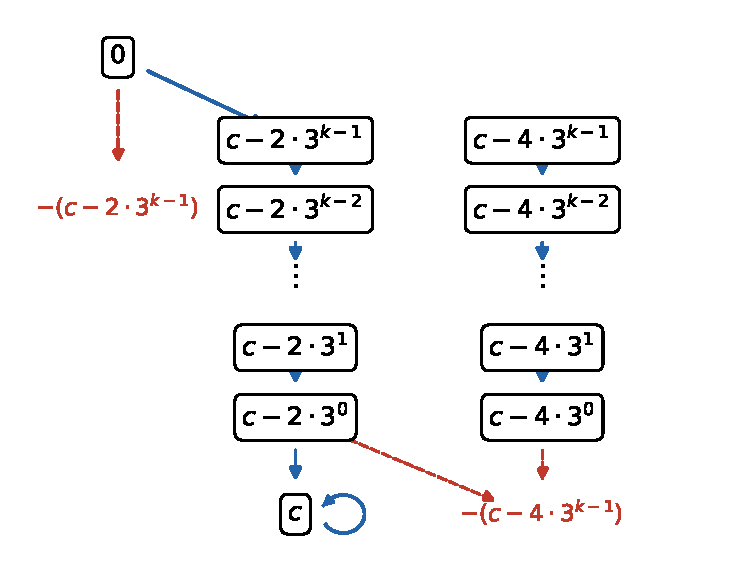
\includegraphics[width=0.75\textwidth]{fig_carries.pdf}
\caption{The positive half of $S_k$ for $n=4\cdot3^k+5$, transcribed from Table~\ref{tab:first}. Solid arrows are moves with $d=1$, dashed arrows moves with $d=-1$ that are not dead; all other moves are dead. The negative half is the mirror image, and its dashed arrows lead back into this half. Every carry reached by a move with $d=1$ has a zero digit, so no path ends in an accepting carry.}
\label{fig:carries}
\end{figure}


\medskip\noindent\emph{Bound.} Every element of $S_k$ has absolute value at most $c=2X+2<n-2$, so (iii)
holds.

\medskip\noindent\emph{No accepting move.} By the table and symmetry, the moves with $d=1$ that are not
dead lead to carries of the form $c$, $c-2\cdot 3^j$ or $c-4\cdot 3^j$ with $0\le j\le k-1$ (the
index $j=k-1$ arises from the moves from $0$, $-(c-2)$ and $-(c-4)$). All of these are positive. Each has a zero
balanced ternary digit, as the following explicit representations show. Write
$c=3^{k+1}-3^k+3-1$.
\begin{itemize}
\item $c$ has nonzero digits only at positions $0,1,k,k+1$, so its digit at position $2$ is $0$.
\item For $2\le j\le k-2$, $c-2\cdot 3^j=c-3^{j+1}+3^j$ and $c-4\cdot 3^j=c-3^{j+1}-3^j$. The six
nonzero digits sit at the distinct positions $0,1,j,j+1,k,k+1$ among the $k+2$ positions
$0,\dots,k+1$, so some digit is $0$ when $k\ge 5$.
\item $c-2=3^{k+1}-3^k$ has digit $0$ at position $0$, and $c-4=3^{k+1}-3^k-3+1$ has digit $0$ at
position $2$.
\item $c-6=3^{k+1}-3^k-3-1$ has digit $0$ at position $2$, and $c-12=3^{k+1}-3^k-3^2-1$ has digit $0$
at position $1$.
\item $c-2\cdot 3^{k-1}=3^k+3^{k-1}+3-1$ and $c-4\cdot 3^{k-1}=3^k-3^{k-1}+3-1$ have digit $0$ at
position $2$.
\end{itemize}
Hence (iv) holds, and Proposition~\ref{prop:criterion} gives $4\cdot 3^k+5\notin\B/\B$ for every
$k\ge 5$. For $k=4$ the second item fails at $j=2$: indeed $329=4\cdot 3^4+5$ lies in $\B/\B$, since
$329\cdot 4=1316$ and $4=(11)_3$, $1316=(1\bar1\bar1 11\bar1 1\bar1)_3$ in balanced ternary with
$\bar1=-1$.

\section{The remaining families}\label{sec:others}

For the remaining families the carry sets are larger and depend on the residue of $k$ modulo $2$ or
$4$, but they have the same shape. Write $X=3^k$. A \emph{chain} is a set
\[
\pm\{\,gX+\beta-t\cdot 3^i : i\in I\,\},
\]
where $g$ is a positive integer, $\beta$ and $t$ are integers, and $I$ is either an interval
$\{\ell\le i\le k-h\}$ (with $h\ge -1$) or the elements of such an interval in a fixed residue
class modulo $2$ or $4$. A \emph{sporadic pair} is a set $\pm\{gX+s\}$ with $g$ a positive rational
whose denominator divides $27$ and $s$ an integer. Appendix~\ref{app:tables} lists, for each family
and each residue class of $k$ concerned, a
set $S_k$ consisting of $0$, a few chains and a few sporadic pairs; in every case $S_k=-S_k$ and
$|S_k|$ is linear in $k$. For example, when $n=4\cdot 3^k-5$,
\[
S_k=\{0\}\cup\pm\Bigl\{\tfrac23X,\ \tfrac23X+2\Bigr\}\cup
\pm\{2X-2-2\cdot 3^i\}_{0\le i\le k-1}\cup\pm\{2X-2-4\cdot 3^i,\ 2X-2-8\cdot 3^i\}_{0\le i\le k-2}.
\]

Conditions (i) and (iii) of Proposition~\ref{prop:criterion} are immediate from the tables. Conditions
(ii) and (iv) reduce to finitely many cases, uniformly in $k$, through the following two observations.

\begin{lemma}[chain step]\label{lem:chain}
Let $n=a\cdot 3^k+b$, let $r=\sigma(gX+\beta-t\cdot 3^i)$ with $\sigma=\pm1$, $i\ge 1$ and $k\ge 1$,
and let $d=\pm 1$. The move $(r,d)$ is dead if and only if $\bal{\sigma\beta+db}=0$. Otherwise it
produces the digit $e=\bal{\sigma\beta+db}$ and leads to
\[
r'=\frac{\sigma g+da}{3}\,X\;-\;\sigma t\cdot 3^{i-1}\;+\;\frac{\sigma\beta+db-e}{3}.
\]
\end{lemma}

\begin{proof}
We have $r+nd=(\sigma g+da)X-\sigma t\cdot 3^i+(\sigma\beta+db)$, and the first two terms are
divisible by $3$.
\end{proof}

So a move from a chain element of index $i\ge 1$ either dies for every such $i$ or lands on the
element of index $i-1$ of a set of the same form, $\pm\{g'X+\beta'-t'\cdot 3^{i}\}$, whose parameters
are determined by $(\sigma,g,\beta,t,d)$ alone (a priori $g'$ is only rational); closure then asks
that this set be one of the chains of $S_k$, or lie in $S_k$ over the relevant indices. Checking (ii) for
all but boundedly many indices therefore amounts to comparing parameters and index ranges. The
remaining moves, from the lowest indices of each chain, from the sporadic pairs and from $0$, are
finitely many explicit computations of the kind in Table~\ref{tab:first}, whose targets have index
$k-j$ or a fixed small index.

\begin{lemma}[gap]\label{lem:gap}
Let $x=H\cdot 3^s+R$ with integers $H$, $R$ and $s\ge 1$. Suppose the balanced ternary digit of
$R$ at some position $p<s$ is $0$ and $|x|>(3^{p+1}-1)/2$. Then $x$ is not zero-free.
\end{lemma}

\begin{proof}
The balanced digit of $x$ at position $p$ depends only on $x$ modulo $3^{p+1}$, and
$x\equiv R\pmod{3^{p+1}}$, so it is $0$. Since $|x|>(3^{p+1}-1)/2$, the representation of $x$ has more
than $p+1$ digits, so this zero is a genuine digit.
\end{proof}

Every positive target of a move with $d=1$ is either $gX+\beta-t\cdot 3^i$ with $i$ large, to which
Lemma~\ref{lem:gap} applies with $s=i$ and $R=\beta$, or $gX+R$ with a fixed integer $R$ (a
sporadic element, or a chain element of small index), to which it applies with $s=k-m$, where $3^m$
is the denominator of $g$ (in our tables $m\le 2$). In each case
$p$ is the position of the first zero digit of $R$, which is at most the length of $R$. This gives
(iv) for all large $k$.

For these families the case analysis is too long to print, and Theorems~\ref{thm:main}
and~\ref{thm:classes} rest on a computer verification of it, in Lean~4 as described in the next
section: symbolically for $k\ge 14$, and for the finitely many $k$ between the lower bound and $13$
through the exact reachable carry set, on which (i) to (iv) are checked directly. For the five
families of Theorem~\ref{thm:main} the symbolic analysis was also carried out independently by a
checker in Python that represents carries as linear forms in $X$ and $3^i$; it treats $k$ by parity
only, so it does not cover the residue classes modulo $4$ of Theorem~\ref{thm:classes}. The sharpness claims follow from explicit witnesses: with $\bar 1=-1$,
\[
319\cdot 4=1276,\qquad 655\cdot 2=1310,\qquad 665\cdot 2=1330
\]
for $4\cdot 3^4-5$, $8\cdot 3^4+7$ and $8\cdot 3^4+17$, where $4=(11)_3$, $2=(1\bar 1)_3$ and
$1276$, $1310$, $1330$ are zero-free; for $8\cdot 3^6-7=5825$ the smallest witness is
$m=8620770364$, with $5825\,m=50215987370300$ zero-free. (The number $8\cdot 3^5-7=1937$ is also an
exception; it is in the list of \cite{BMRS}, but it is not covered by the uniform argument.)

\section{Formal verification}\label{sec:lean}

All thirteen results of Theorems~\ref{thm:main} and~\ref{thm:classes} are proved in Lean~4 \cite{Lean4} (version 4.34, core library
only, without Mathlib). The statement proved for $8\cdot 3^k+17$, for example, is
\[
\forall k\ge 5,\quad \neg\,\exists\, m,N\in\Z,\ \ 0<m\ \wedge\ \mathtt{ZF}\,m\ \wedge\ 0<N\ \wedge\
\mathtt{ZF}\,N\ \wedge\ N=(8\cdot 3^k+17)\,m,
\]
where \texttt{ZF} is defined inductively: $1$ and $-1$ are zero-free, and if $q$ is zero-free then so
are $3q\pm1$. The development has three layers.
\begin{enumerate}
\item A shared file proves Proposition~\ref{prop:criterion} for an arbitrary predicate $S$, and a
second version for a concrete finite list of carries, whose conditions are checked by a Boolean
function with a proved soundness lemma, so that a concrete instance is closed by evaluation
(\texttt{decide}).
\item For each family and each residue class of $k$, the set $S_k$ is an inductive predicate with one
constructor per chain or sporadic pair. Closure is proved constructor by constructor: the lowest
indices are split off explicitly, the generic index is sent to $i-1$ as in Lemma~\ref{lem:chain},
and every resulting identity or congruence is discharged by the decision procedure \texttt{omega}
for linear integer arithmetic, with the powers $3^k,3^{k-1},\dots$ and $3^i,3^{i-1},\dots$ as
atoms tied together by the equations $3^{x+1}=3\cdot 3^x$. The absence of positive zero-free
carries is proved by peeling digits as in Lemma~\ref{lem:gap}. These lemmas hold for all $k\ge 14$.
\item The values of $k$ from the lower bound up to $13$ are handled by concrete certificates: the
exact reachable carry set, checked by evaluation.
\end{enumerate}
The proof scripts for all but the first family were produced by a program that reads the carry sets
of Appendix~\ref{app:tables} and decides, for each case, which constructor and index the move lands
on. The program's choices are not trusted: Lean re-checks each one, so an incorrect choice makes the
file fail to compile. The thirteen main theorems depend only on the standard axioms \texttt{propext},
\texttt{Quot.sound} and \texttt{Classical.choice}; there is no \texttt{sorry} and no use of
\texttt{native\_decide}. The whole development (about $31{,}000$ lines, most of them generated)
compiles in about three minutes on a laptop. As a check that the verification can fail, we compiled
eight corrupted versions: claiming the result for $8\cdot 3^k+19$ or for $40\cdot 3^k+43$, changing a
chain coefficient throughout (in two families), extending $4\cdot 3^k-5$ to $k=4$ or $5\cdot 3^k+4$ to
$k=4$, shifting a sporadic carry, and claiming $5\cdot 3^k+4\notin\B/\B$ for $k\equiv 1\pmod 4$. Each
was rejected. A hand-written Lean proof of the case $4\cdot 3^k+5$, following
Section~\ref{sec:first}, was also checked separately.

\section{Digits \texorpdfstring{$0$}{0} and \texorpdfstring{$1$}{1}}\label{sec:cantor}

Guy's entry F31 also asks which integers are quotients of numbers written in base $3$ with the digits
$0$ and $1$ only. Following \cite{BMRS}, let $C$ be this set of positive integers,
$V=\N\cap C/C$,
\[
D=\{N : N\equiv 2\cdot 3^{i-1}\pmod{3^i}\text{ for some }i\ge 1\},\qquad
E=\N\cap\bigcup_{i\ge 0}\bigl[\tfrac32\cdot 3^i,\,2\cdot 3^i\bigr],
\]
and $F=\N\setminus(V\cup D\cup E)$. Bai et al.\ show, by looking at numerators and denominators modulo
$3^i$ and at their leading digits, that elements of $D\cup E$ do not lie in $V$, and they report that
Haque and Shallit found the elements
\[
529,\ 592,\ 601,\ 616,\ 5368,\ 50281,\ 4072741,\ 4074361,\ 4088941,\ 4245688
\]
of $F$, asking whether $F$ is infinite and suggesting that $621\cdot 3^{4k}-20$ might always lie in $F$.
Anders, Dawsey, Reznick and Sisneros-Thiry \cite{ADRS} study the same set and report that these ten are
the only elements congruent to $1$ modulo $3$ below $6.2\cdot 10^6$, and that Haque and Shallit found
eleven below $1.07\cdot 10^8$. The OEIS entry A339636 \cite{OEIS} lists the elements up to
$3.44\cdot 10^8$ (computed by R.~Dougherty-Bliss); it includes $621\cdot 3^{12}-20=330024841$, the case
$k=3$ of the guess, whose cases $k=1,2$ are $50281$ and $4074361$. (Only elements congruent to $1$
modulo $3$ need listing, since $V$, $D$ and $E$ are invariant under $N\mapsto 3N$ and $N\mapsto N/3$,
and numbers congruent to $2$ modulo $3$ lie in $D$.)

The carry automaton of Section~\ref{sec:auto}, with digits $0,1$ in place of $\pm1$, decides
membership in $V$ exactly: the proof of Proposition~\ref{prop:criterion} and the remark after it carry
over word for word, with a move dead when its output digit would be $2$ and with acceptance at a
carry that is $0$ or has only the digits $0$ and $1$. The carries stay between $0$ and $n/2$, so the
search is finite. Running it on the next case gives one new data point.

\begin{proposition}\label{prop:cantor}
$621\cdot 3^{16}-20=26732013721$ lies in $F$.
\end{proposition}

The number of reachable carries for $621\cdot 3^{4k}-20$ is $870$, $14368$, $230658$ and $3691740$ for
$k=1,\dots,4$, growing by a factor close to $16=2^4$ per step, that is, like $N^{\log 2/\log 3}$. This
Cantor-type growth is why the chain method of Section~\ref{sec:others}, which relies on carry sets of
linear size, does not apply directly to this family, and we do not claim a proof for all $k$.

\section{Data and questions}\label{sec:data}

A search with the decision procedure of Section~\ref{sec:auto} finds exactly $200$ integers
$n\not\equiv 0\pmod 3$ below $10^8$ outside $\B/\B$. Of these, $136$ fall into $21$ families
$a\cdot 3^k+b$ with at least three members each, listed in Table~\ref{tab:fam}; the other $64$ belong to no
family with $a,|b|\le 300$ and at least three members below $10^8$. Within its range, each family is
periodic in $k$ from some point on, with period $1$, $2$ or $4$. The families also come in visible pairs:
$b$ changes sign, as with $4\cdot 3^k\pm 5$, or the roles of $a$ and $b$ swap, as with $40\cdot 3^k\pm 41$
and $41\cdot 3^k\pm 40$. Theorems~\ref{thm:main} and~\ref{thm:classes} account for every exception in ten of the
families within this range, apart from $1937=8\cdot 3^5-7$, which is known only by computation, and
for three more families on one residue class. For the remaining eight, and for
$5\cdot 3^k\pm 4$ on the other residue classes, we found no carry set of linear size. For
$5\cdot 3^k\pm 4$ the reachable carry sets grow roughly quadratically in $k$, which suggests elements with
two independent indices. For $3^k\pm 4$, $7\cdot 3^k\pm 8$ and $19\cdot 3^k-10$ they grow by a factor of
about $15$ each time $k$ increases by $4$, like the Cantor-type growth of Section~\ref{sec:cantor}. For
$40\cdot 3^k-41$ and $41\cdot 3^k\pm 40$ they have thousands of elements already for $k$ near $13$.
Proving these families needs a different description of the carries.

\begin{table}[htbp]\centering\small
\caption{Families $a\cdot 3^k+b$ among the $200$ exceptions below $10^8$. The pattern shows $k=1,2,\dots$
up to $a\cdot 3^k+b<10^8$: x marks an exception, a dot a member of $\B/\B$.}
\label{tab:fam}
\begin{tabular}{lll}\toprule
family & pattern & \\ \midrule
$4\cdot 3^k-5$ & \texttt{....xxxxxxxxxxx} & proved \\
$4\cdot 3^k+5$ & \texttt{....xxxxxxxxxxx} & proved \\
$5\cdot 3^k-4$ & \texttt{....xxxxxxxxxxx} & proved for $k\equiv 2\ (4)$ \\
$5\cdot 3^k+4$ & \texttt{....xxxxxxxxxxx} & proved for $k\equiv 0\ (4)$ \\
$8\cdot 3^k+7$ & \texttt{....xxxxxxxxxx} & proved \\
$8\cdot 3^k+17$ & \texttt{....xxxxxxxxxx} & proved \\
$8\cdot 3^k-7$ & \texttt{....x.xxxxxxxx} & proved for $k\ge 7$ \\
$3^k+4$ & \texttt{....x.x.x.x.x.x.} &  \\
$3^k-4$ & \texttt{~.....x.x.x.x.x.} &  \\
$7\cdot 3^k-8$ & \texttt{.....x.x.x.x.x} &  \\
$7\cdot 3^k+8$ & \texttt{.....x.x.x.x.x} &  \\
$8\cdot 3^k-17$ & \texttt{.....x.x.x.x.x} & proved \\
$16\cdot 3^k+17$ & \texttt{.....x.x.x.x.x} & proved \\
$40\cdot 3^k-41$ & \texttt{........xxxxx} &  \\
$40\cdot 3^k+41$ & \texttt{........xxxxx} & proved for $k\equiv 0\ (4)$ \\
$41\cdot 3^k-40$ & \texttt{........xxxxx} &  \\
$41\cdot 3^k+40$ & \texttt{........xxxxx} &  \\
$10\cdot 3^k-19$ & \texttt{.....x...x...x} & proved \\
$10\cdot 3^k-11$ & \texttt{.....x...x...x} & proved \\
$19\cdot 3^k-10$ & \texttt{.....x...x...x} &  \\
$20\cdot 3^k-19$ & \texttt{.....x...x...x} & proved \\
\bottomrule\end{tabular}\end{table}

\begin{question}
Is $5\cdot 3^k+4\notin\B/\B$ for all $k\ge 5$? Is $3^k+4\notin\B/\B$ for all odd $k\ge 5$?
\end{question}

\begin{question}
Does $\B/\B$ contain almost all integers prime to $3$, that is, do the exceptions have density zero?
\end{question}

\begin{question}
Is $F$ infinite? In particular, is $621\cdot 3^{4k}-20\in F$ for every $k\ge 1$?
\end{question}

\section*{Code and data}
The Lean development, the program that generates it, the decision procedures, the list of the $200$
exceptions below $10^8$, and a program that recomputes every number quoted in this paper are at
\begin{center}\small\url{https://github.com/jvvk/mathematics/tree/main/balanced-ternary-quotients}.\end{center}

\section*{Declaration of generative AI use}
The author used Claude (Anthropic; Claude Opus models, between 19 September and 8 October 2026)
throughout this work, under the author's direction: to run the searches for exceptions and fit the carry sets
of Appendix~\ref{app:tables}, to write the decision programs, the symbolic checker, the program that
generates the Lean proofs and the hand-written Lean proof, to search the literature, and to draft the
text. The reason was to obtain a computer-assisted proof that can be checked in full: every theorem
is verified in Lean (Section~\ref{sec:lean}), and every number quoted is recomputed by a separate
program (see \emph{Code and data}). The author takes full responsibility for the content, including
the references.

\begin{thebibliography}{9}

\bibitem{BMRS}
J.~H.~Bai, J.~Meleshko, S.~Riasat and J.~Shallit,
Quotients of palindromic and antipalindromic numbers,
\emph{Integers} \textbf{22} (2022), Paper A96,
\url{https://math.colgate.edu/~integers/w96/w96.pdf}; arXiv:2202.13694.

\bibitem{ADRS}
K.~Anders, M.~L.~Dawsey, B.~Reznick and S.~Sisneros-Thiry,
Representations of integers as quotients of sums of distinct powers of three,
arXiv:2308.07252, 2023.

\bibitem{Guy04}
R.~K.~Guy,
\emph{Unsolved Problems in Number Theory}, 3rd edition, Problem Books in Mathematics, Springer,
New York, 2004, \href{https://doi.org/10.1007/978-0-387-26677-0}{doi:10.1007/978-0-387-26677-0}.

\bibitem{LvdP}
J.~H.~Loxton and A.~J.~van der Poorten,
An awful problem about integers in base four,
\emph{Acta Arith.} \textbf{49} (1987), no.~2, 193--203,
\href{https://doi.org/10.4064/aa-49-2-193-203}{doi:10.4064/aa-49-2-193-203}.

\bibitem{RS}
E.~Rowland and J.~Shallit,
Automatic sets of rational numbers,
\emph{Internat.\ J. Found.\ Comput.\ Sci.} \textbf{26} (2015), no.~3, 343--365,
\href{https://doi.org/10.1142/S0129054115500197}{doi:10.1142/S0129054115500197}.

\bibitem{OEIS}
OEIS Foundation Inc., The On-Line Encyclopedia of Integer Sequences, \url{https://oeis.org},
entries A339636 and A351243, accessed 8 October 2026.

\bibitem{Lean4}
L.~de Moura and S.~Ullrich,
The Lean 4 theorem prover and programming language,
in \emph{Automated Deduction, CADE 28}, Lecture Notes in Comput.\ Sci.\ \textbf{12699}, Springer, 2021,
625--635, \href{https://doi.org/10.1007/978-3-030-79876-5_37}{doi:10.1007/978-3-030-79876-5\_37}.

\end{thebibliography}

\appendix
\section{Carry sets}\label{app:tables}

In each table $X=3^k$, and every row stands for the listed element together with its negative. The
sizes $|S_k|$ are for $k\ge 14$ in the stated parity class.

\begin{table}[htbp]\centering\small
\caption{Carry set $S_k$ for $n=4\cdot 3^k - 5$, all $k$; $X=3^k$, $|S_k|=6k+1$.}
\label{tab:4m50}
\begin{tabular}{ll}\toprule
element & index range \\ \midrule
$0$ & \\
$\pm\bigl(2X - 2 - 8\cdot 3^i\bigr)$ & $0\le i\le k-2$ \\
$\pm\bigl(2X - 2 - 2\cdot 3^i\bigr)$ & $0\le i\le k-1$ \\
$\pm\bigl(2X - 2 - 4\cdot 3^i\bigr)$ & $0\le i\le k-2$ \\
$\pm\bigl(\tfrac{2}{3}X\bigr)$ & sporadic \\
$\pm\bigl(\tfrac{2}{3}X + 2\bigr)$ & sporadic \\
\bottomrule\end{tabular}\end{table}

\begin{table}[htbp]\centering\small
\caption{Carry set $S_k$ for $n=8\cdot 3^k + 7$, $k$ even; $X=3^k$, $|S_k|=4k+3$.}
\label{tab:8p70}
\begin{tabular}{ll}\toprule
element & index range \\ \midrule
$0$ & \\
$\pm\bigl(2X + 2 - 2\cdot 3^i\bigr)$ & $0\le i\le k-2$, $i\equiv 0\pmod 2$ \\
$\pm\bigl(2X + 2 - 4\cdot 3^i\bigr)$ & $0\le i\le k-2$, $i\equiv 0\pmod 2$ \\
$\pm\bigl(2X + 2 + 4\cdot 3^i\bigr)$ & $1\le i\le k-1$, $i\equiv 1\pmod 2$ \\
$\pm\bigl(2X + 2 + 2\cdot 3^i\bigr)$ & $1\le i\le k-1$, $i\equiv 1\pmod 2$ \\
$\pm\bigl(2X + 2\bigr)$ & sporadic \\
\bottomrule\end{tabular}\end{table}

\begin{table}[htbp]\centering\small
\caption{Carry set $S_k$ for $n=8\cdot 3^k + 7$, $k$ odd; $X=3^k$, $|S_k|=8k+3$.}
\label{tab:8p71}
\begin{tabular}{ll}\toprule
element & index range \\ \midrule
$0$ & \\
$\pm\bigl(2X + 2 - 2\cdot 3^i\bigr)$ & $0\le i\le k-1$ \\
$\pm\bigl(2X + 2 + 4\cdot 3^i\bigr)$ & $0\le i\le k-1$, $i\equiv 0\pmod 2$ \\
$\pm\bigl(2X + 2 - 4\cdot 3^i\bigr)$ & $1\le i\le k-2$, $i\equiv 1\pmod 2$ \\
$\pm\bigl(2X + 2 + 2\cdot 3^i\bigr)$ & $0\le i\le k$ \\
$\pm\bigl(4X + 4 - 2\cdot 3^i\bigr)$ & $1\le i\le k-1$ \\
$\pm\bigl(2X + 2\bigr)$ & sporadic \\
\bottomrule\end{tabular}\end{table}

\begin{table}[htbp]\centering\small
\caption{Carry set $S_k$ for $n=8\cdot 3^k + 17$, $k$ even; $X=3^k$, $|S_k|=10k+3$.}
\label{tab:8p170}
\begin{tabular}{ll}\toprule
element & index range \\ \midrule
$0$ & \\
$\pm\bigl(2X + 4 - 2\cdot 3^i\bigr)$ & $0\le i\le k-1$ \\
$\pm\bigl(2X + 4 - 4\cdot 3^i\bigr)$ & $0\le i\le k-2$, $i\equiv 0\pmod 2$ \\
$\pm\bigl(2X + 4 + 4\cdot 3^i\bigr)$ & $1\le i\le k-3$, $i\equiv 1\pmod 2$ \\
$\pm\bigl(2X + 4 + 2\cdot 3^i\bigr)$ & $0\le i\le k$, $i\equiv 0\pmod 2$ \\
$\pm\bigl(2X + 4 + 2\cdot 3^i\bigr)$ & $1\le i\le k-3$, $i\equiv 1\pmod 2$ \\
$\pm\bigl(4X + 8 - 2\cdot 3^i\bigr)$ & $0\le i\le k-1$ \\
$\pm\bigl(4X + 8 - 4\cdot 3^i\bigr)$ & $1\le i\le k-2$ \\
$\pm\bigl(2X + 4\bigr)$ & sporadic \\
$\pm\bigl(\tfrac{8}{3}X + 6\bigr)$ & sporadic \\
$\pm\bigl(\tfrac{10}{3}X + 6\bigr)$ & sporadic \\
$\pm\bigl(4X + 8\bigr)$ & sporadic \\
\bottomrule\end{tabular}\end{table}

\begin{table}[htbp]\centering\small
\caption{Carry set $S_k$ for $n=8\cdot 3^k + 17$, $k$ odd; $X=3^k$, $|S_k|=10k+3$.}
\label{tab:8p171}
\begin{tabular}{ll}\toprule
element & index range \\ \midrule
$0$ & \\
$\pm\bigl(2X + 4 - 2\cdot 3^i\bigr)$ & $0\le i\le k-1$ \\
$\pm\bigl(2X + 4 + 4\cdot 3^i\bigr)$ & $0\le i\le k-3$, $i\equiv 0\pmod 2$ \\
$\pm\bigl(2X + 4 - 4\cdot 3^i\bigr)$ & $1\le i\le k-2$, $i\equiv 1\pmod 2$ \\
$\pm\bigl(2X + 4 + 2\cdot 3^i\bigr)$ & $0\le i\le k-3$, $i\equiv 0\pmod 2$ \\
$\pm\bigl(2X + 4 + 2\cdot 3^i\bigr)$ & $1\le i\le k$, $i\equiv 1\pmod 2$ \\
$\pm\bigl(4X + 8 - 2\cdot 3^i\bigr)$ & $0\le i\le k-1$ \\
$\pm\bigl(4X + 8 - 4\cdot 3^i\bigr)$ & $1\le i\le k-2$ \\
$\pm\bigl(2X + 4\bigr)$ & sporadic \\
$\pm\bigl(\tfrac{8}{3}X + 6\bigr)$ & sporadic \\
$\pm\bigl(\tfrac{10}{3}X + 6\bigr)$ & sporadic \\
$\pm\bigl(4X + 8\bigr)$ & sporadic \\
\bottomrule\end{tabular}\end{table}

\begin{table}[htbp]\centering\small
\caption{Carry set $S_k$ for $n=8\cdot 3^k - 7$, $k$ even; $X=3^k$, $|S_k|=12k+5$.}
\label{tab:8m70}
\begin{tabular}{ll}\toprule
element & index range \\ \midrule
$0$ & \\
$\pm\bigl(2X - 2 - 2\cdot 3^i\bigr)$ & $0\le i\le k-2$ \\
$\pm\bigl(2X - 2 - 4\cdot 3^i\bigr)$ & $0\le i\le k-2$, $i\equiv 0\pmod 2$ \\
$\pm\bigl(2X - 2 - 10\cdot 3^i\bigr)$ & $1\le i\le k-3$, $i\equiv 1\pmod 2$ \\
$\pm\bigl(2X - 2 + 16\cdot 3^i\bigr)$ & $0\le i\le k-2$, $i\equiv 0\pmod 2$ \\
$\pm\bigl(2X - 2 - 16\cdot 3^i\bigr)$ & $1\le i\le k-3$, $i\equiv 1\pmod 2$ \\
$\pm\bigl(2X - 2 + 10\cdot 3^i\bigr)$ & $0\le i\le k-2$, $i\equiv 0\pmod 2$ \\
$\pm\bigl(2X - 2 + 4\cdot 3^i\bigr)$ & $1\le i\le k-1$, $i\equiv 1\pmod 2$ \\
$\pm\bigl(2X - 2 + 2\cdot 3^i\bigr)$ & $0\le i\le k-1$ \\
$\pm\bigl(4X - 4 - 2\cdot 3^i\bigr)$ & $0\le i\le k-1$ \\
$\pm\bigl(\tfrac{4}{3}X\bigr)$ & sporadic \\
$\pm\bigl(2X - 2\bigr)$ & sporadic \\
$\pm\bigl(\tfrac{10}{3}X\bigr)$ & sporadic \\
$\pm\bigl(\tfrac{10}{3}X + 2\bigr)$ & sporadic \\
$\pm\bigl(4X - 4\bigr)$ & sporadic \\
\bottomrule\end{tabular}\end{table}

\begin{table}[htbp]\centering\small
\caption{Carry set $S_k$ for $n=8\cdot 3^k - 7$, $k$ odd; $X=3^k$, $|S_k|=4k+3$.}
\label{tab:8m71}
\begin{tabular}{ll}\toprule
element & index range \\ \midrule
$0$ & \\
$\pm\bigl(2X - 2 - 2\cdot 3^i\bigr)$ & $1\le i\le k-2$, $i\equiv 1\pmod 2$ \\
$\pm\bigl(2X - 2 + 4\cdot 3^i\bigr)$ & $0\le i\le k-1$, $i\equiv 0\pmod 2$ \\
$\pm\bigl(2X - 2 - 4\cdot 3^i\bigr)$ & $1\le i\le k-2$, $i\equiv 1\pmod 2$ \\
$\pm\bigl(2X - 2 + 2\cdot 3^i\bigr)$ & $0\le i\le k-1$, $i\equiv 0\pmod 2$ \\
$\pm\bigl(2X - 2\bigr)$ & sporadic \\
\bottomrule\end{tabular}\end{table}

\begin{table}[htbp]\centering\small
\caption{Carry set $S_k$ for $n=8\cdot 3^k - 17$, $k\equiv 0\pmod{2}$; $X=3^k$, $|S_k|=16k-3$.}
\begin{tabular}{ll}\toprule
element & index range \\ \midrule
$0$ & \\
$\pm\bigl(4X - 8 - 8\cdot 3^i\bigr)$ & $0\le i\le k-3$ \\
$\pm\bigl(4X - 8 - 16\cdot 3^i\bigr)$ & $0\le i\le k-3$ \\
$\pm\bigl(4X - 8 - 2\cdot 3^i\bigr)$ & $0\le i\le k$ \\
$\pm\bigl(4X - 8 - 4\cdot 3^i\bigr)$ & $0\le i\le k-2$ \\
$\pm\bigl(2X - 4 - 2\cdot 3^i\bigr)$ & $0\le i\le k-2$ \\
$\pm\bigl(2X - 4 - 4\cdot 3^i\bigr)$ & $2\le i\le k-2$, $i\equiv 0\pmod 2$ \\
$\pm\bigl(2X - 4 - 10\cdot 3^i\bigr)$ & $1\le i\le k-3$, $i\equiv 1\pmod 2$ \\
$\pm\bigl(2X - 4 + 10\cdot 3^i\bigr)$ & $0\le i\le k-4$, $i\equiv 0\pmod 2$ \\
$\pm\bigl(2X - 4 + 4\cdot 3^i\bigr)$ & $1\le i\le k-1$, $i\equiv 1\pmod 2$ \\
$\pm\bigl(2X - 4 + 2\cdot 3^i\bigr)$ & $0\le i\le k-3$ \\
$\pm\bigl(\tfrac{4}{3}X - 2\bigr)$ & sporadic \\
$\pm\bigl(\tfrac{4}{3}X\bigr)$ & sporadic \\
$\pm\bigl(\tfrac{4}{3}X + 2\bigr)$ & sporadic \\
$\pm\bigl(2X - 4\bigr)$ & sporadic \\
$\pm\bigl(\tfrac{20}{9}X - 6\bigr)$ & sporadic \\
$\pm\bigl(\tfrac{8}{3}X - 6\bigr)$ & sporadic \\
$\pm\bigl(\tfrac{28}{9}X - 6\bigr)$ & sporadic \\
$\pm\bigl(\tfrac{10}{3}X - 6\bigr)$ & sporadic \\
\bottomrule\end{tabular}\end{table}

\begin{table}[htbp]\centering\small
\caption{Carry set $S_k$ for $n=16\cdot 3^k + 17$, $k\equiv 0\pmod{2}$; $X=3^k$, $|S_k|=12k+11$.}
\begin{tabular}{ll}\toprule
element & index range \\ \midrule
$0$ & \\
$\pm\bigl(4X + 4 - 4\cdot 3^i\bigr)$ & $0\le i\le k-1$ \\
$\pm\bigl(4X + 4 - 8\cdot 3^i\bigr)$ & $0\le i\le k-2$, $i\equiv 0\pmod 2$ \\
$\pm\bigl(4X + 4 + 8\cdot 3^i\bigr)$ & $1\le i\le k-1$, $i\equiv 1\pmod 2$ \\
$\pm\bigl(4X + 4 + 4\cdot 3^i\bigr)$ & $0\le i\le k$, $i\equiv 0\pmod 2$ \\
$\pm\bigl(4X + 4 + 4\cdot 3^i\bigr)$ & $1\le i\le k-3$, $i\equiv 1\pmod 2$ \\
$\pm\bigl(8X + 8 - 8\cdot 3^i\bigr)$ & $0\le i\le k-2$ \\
$\pm\bigl(8X + 8 - 16\cdot 3^i\bigr)$ & $0\le i\le k-1$ \\
$\pm\bigl(8X + 8 - 4\cdot 3^i\bigr)$ & $1\le i\le k-1$ \\
$\pm\bigl(\tfrac{8}{3}X + 6\bigr)$ & sporadic \\
$\pm\bigl(4X + 4\bigr)$ & sporadic \\
$\pm\bigl(4X + 6\bigr)$ & sporadic \\
$\pm\bigl(\tfrac{16}{3}X + 6\bigr)$ & sporadic \\
$\pm\bigl(\tfrac{20}{3}X + 6\bigr)$ & sporadic \\
$\pm\bigl(8X + 6\bigr)$ & sporadic \\
$\pm\bigl(8X + 8\bigr)$ & sporadic \\
\bottomrule\end{tabular}\end{table}

\begin{table}[htbp]\centering\small
\caption{Carry set $S_k$ for $n=10\cdot 3^k - 11$, $k\equiv 2\pmod{4}$; $X=3^k$, $|S_k|=4k+5$.}
\begin{tabular}{ll}\toprule
element & index range \\ \midrule
$0$ & \\
$\pm\bigl(2X - 2 - 2\cdot 3^i\bigr)$ & $2\le i\le k-4$, $i\equiv 2\pmod 4$ \\
$\pm\bigl(2X - 2 + 4\cdot 3^i\bigr)$ & $0\le i\le k-2$, $i\equiv 0\pmod 4$ \\
$\pm\bigl(2X - 2 - 4\cdot 3^i\bigr)$ & $2\le i\le k-4$, $i\equiv 2\pmod 4$ \\
$\pm\bigl(2X - 2 + 2\cdot 3^i\bigr)$ & $0\le i\le k-2$, $i\equiv 0\pmod 4$ \\
$\pm\bigl(4X - 4 - 2\cdot 3^i\bigr)$ & $1\le i\le k-1$, $i\equiv 1\pmod 4$ \\
$\pm\bigl(4X - 4 - 4\cdot 3^i\bigr)$ & $1\le i\le k-1$, $i\equiv 1\pmod 4$ \\
$\pm\bigl(4X - 4 + 4\cdot 3^i\bigr)$ & $3\le i\le k-3$, $i\equiv 3\pmod 4$ \\
$\pm\bigl(4X - 4 + 2\cdot 3^i\bigr)$ & $3\le i\le k-3$, $i\equiv 3\pmod 4$ \\
$\pm\bigl(2X - 2\bigr)$ & sporadic \\
$\pm\bigl(4X - 4\bigr)$ & sporadic \\
\bottomrule\end{tabular}\end{table}

\begin{table}[htbp]\centering\small
\caption{Carry set $S_k$ for $n=10\cdot 3^k - 19$, $k\equiv 2\pmod{4}$; $X=3^k$, $|S_k|=10k+3$.}
\begin{tabular}{ll}\toprule
element & index range \\ \midrule
$0$ & \\
$\pm\bigl(2X - 4 - 2\cdot 3^i\bigr)$ & $0\le i\le k-2$, $i\equiv 0\pmod 4$ \\
$\pm\bigl(2X - 4 - 2\cdot 3^i\bigr)$ & $2\le i\le k-4$, $i\equiv 2\pmod 4$ \\
$\pm\bigl(2X - 4 - 2\cdot 3^i\bigr)$ & $3\le i\le k-3$, $i\equiv 3\pmod 4$ \\
$\pm\bigl(2X - 4 + 4\cdot 3^i\bigr)$ & $0\le i\le k-2$, $i\equiv 0\pmod 4$ \\
$\pm\bigl(2X - 4 + 4\cdot 3^i\bigr)$ & $1\le i\le k-5$, $i\equiv 1\pmod 4$ \\
$\pm\bigl(2X - 4 - 4\cdot 3^i\bigr)$ & $2\le i\le k-4$, $i\equiv 2\pmod 4$ \\
$\pm\bigl(2X - 4 - 4\cdot 3^i\bigr)$ & $3\le i\le k-3$, $i\equiv 3\pmod 4$ \\
$\pm\bigl(2X - 4 + 2\cdot 3^i\bigr)$ & $0\le i\le k-2$, $i\equiv 0\pmod 4$ \\
$\pm\bigl(2X - 4 + 2\cdot 3^i\bigr)$ & $1\le i\le k-1$, $i\equiv 1\pmod 4$ \\
$\pm\bigl(2X - 4 + 2\cdot 3^i\bigr)$ & $2\le i\le k$, $i\equiv 2\pmod 4$ \\
$\pm\bigl(4X - 8 - 2\cdot 3^i\bigr)$ & $1\le i\le k-5$, $i\equiv 1\pmod 4$ \\
$\pm\bigl(4X - 8 - 2\cdot 3^i\bigr)$ & $2\le i\le k-4$, $i\equiv 2\pmod 4$ \\
$\pm\bigl(4X - 8 - 2\cdot 3^i\bigr)$ & $3\le i\le k-3$, $i\equiv 3\pmod 4$ \\
$\pm\bigl(4X - 8 - 4\cdot 3^i\bigr)$ & $1\le i\le k-5$, $i\equiv 1\pmod 4$ \\
$\pm\bigl(4X - 8 - 4\cdot 3^i\bigr)$ & $2\le i\le k-4$, $i\equiv 2\pmod 4$ \\
$\pm\bigl(4X - 8 + 4\cdot 3^i\bigr)$ & $4\le i\le k-2$, $i\equiv 0\pmod 4$ \\
$\pm\bigl(4X - 8 + 4\cdot 3^i\bigr)$ & $3\le i\le k-3$, $i\equiv 3\pmod 4$ \\
$\pm\bigl(4X - 8 + 2\cdot 3^i\bigr)$ & $0\le i\le k-2$, $i\equiv 0\pmod 4$ \\
$\pm\bigl(4X - 8 + 2\cdot 3^i\bigr)$ & $1\le i\le k-1$, $i\equiv 1\pmod 4$ \\
$\pm\bigl(4X - 8 + 2\cdot 3^i\bigr)$ & $3\le i\le k-3$, $i\equiv 3\pmod 4$ \\
$\pm\bigl(2X - 4\bigr)$ & sporadic \\
$\pm\bigl(\tfrac{8}{3}X - 6\bigr)$ & sporadic \\
$\pm\bigl(\tfrac{10}{3}X - 6\bigr)$ & sporadic \\
$\pm\bigl(4X - 8\bigr)$ & sporadic \\
\bottomrule\end{tabular}\end{table}

\begin{table}[htbp]\centering\small
\caption{Carry set $S_k$ for $n=20\cdot 3^k - 19$, $k\equiv 2\pmod{4}$; $X=3^k$, $|S_k|=12k+11$.}
\begin{tabular}{ll}\toprule
element & index range \\ \midrule
$0$ & \\
$\pm\bigl(4X - 4 - 4\cdot 3^i\bigr)$ & $0\le i\le k-2$, $i\equiv 0\pmod 4$ \\
$\pm\bigl(4X - 4 - 4\cdot 3^i\bigr)$ & $2\le i\le k-4$, $i\equiv 2\pmod 4$ \\
$\pm\bigl(4X - 4 - 4\cdot 3^i\bigr)$ & $3\le i\le k-3$, $i\equiv 3\pmod 4$ \\
$\pm\bigl(4X - 4 - 8\cdot 3^i\bigr)$ & $2\le i\le k-4$, $i\equiv 2\pmod 4$ \\
$\pm\bigl(4X - 4 - 8\cdot 3^i\bigr)$ & $3\le i\le k-3$, $i\equiv 3\pmod 4$ \\
$\pm\bigl(4X - 4 + 16\cdot 3^i\bigr)$ & $1\le i\le k-1$, $i\equiv 1\pmod 4$ \\
$\pm\bigl(4X - 4 - 16\cdot 3^i\bigr)$ & $3\le i\le k-3$, $i\equiv 3\pmod 4$ \\
$\pm\bigl(4X - 4 + 8\cdot 3^i\bigr)$ & $0\le i\le k-2$, $i\equiv 0\pmod 4$ \\
$\pm\bigl(4X - 4 + 8\cdot 3^i\bigr)$ & $1\le i\le k-5$, $i\equiv 1\pmod 4$ \\
$\pm\bigl(4X - 4 + 4\cdot 3^i\bigr)$ & $0\le i\le k-2$, $i\equiv 0\pmod 4$ \\
$\pm\bigl(4X - 4 + 4\cdot 3^i\bigr)$ & $1\le i\le k-1$, $i\equiv 1\pmod 4$ \\
$\pm\bigl(4X - 4 + 4\cdot 3^i\bigr)$ & $2\le i\le k$, $i\equiv 2\pmod 4$ \\
$\pm\bigl(8X - 8 - 4\cdot 3^i\bigr)$ & $1\le i\le k-5$, $i\equiv 1\pmod 4$ \\
$\pm\bigl(8X - 8 - 4\cdot 3^i\bigr)$ & $2\le i\le k-4$, $i\equiv 2\pmod 4$ \\
$\pm\bigl(8X - 8 - 4\cdot 3^i\bigr)$ & $3\le i\le k-3$, $i\equiv 3\pmod 4$ \\
$\pm\bigl(8X - 8 - 8\cdot 3^i\bigr)$ & $1\le i\le k-1$, $i\equiv 1\pmod 4$ \\
$\pm\bigl(8X - 8 - 8\cdot 3^i\bigr)$ & $2\le i\le k-4$, $i\equiv 2\pmod 4$ \\
$\pm\bigl(8X - 8 + 16\cdot 3^i\bigr)$ & $0\le i\le k-2$, $i\equiv 0\pmod 4$ \\
$\pm\bigl(8X - 8 - 16\cdot 3^i\bigr)$ & $2\le i\le k-4$, $i\equiv 2\pmod 4$ \\
$\pm\bigl(8X - 8 + 8\cdot 3^i\bigr)$ & $0\le i\le k-2$, $i\equiv 0\pmod 4$ \\
$\pm\bigl(8X - 8 + 8\cdot 3^i\bigr)$ & $3\le i\le k-3$, $i\equiv 3\pmod 4$ \\
$\pm\bigl(8X - 8 + 4\cdot 3^i\bigr)$ & $4\le i\le k-2$, $i\equiv 0\pmod 4$ \\
$\pm\bigl(8X - 8 + 4\cdot 3^i\bigr)$ & $1\le i\le k-1$, $i\equiv 1\pmod 4$ \\
$\pm\bigl(8X - 8 + 4\cdot 3^i\bigr)$ & $3\le i\le k-3$, $i\equiv 3\pmod 4$ \\
$\pm\bigl(4X - 6\bigr)$ & sporadic \\
$\pm\bigl(4X - 4\bigr)$ & sporadic \\
$\pm\bigl(\tfrac{16}{3}X - 6\bigr)$ & sporadic \\
$\pm\bigl(\tfrac{20}{3}X - 6\bigr)$ & sporadic \\
$\pm\bigl(8X - 8\bigr)$ & sporadic \\
$\pm\bigl(8X - 6\bigr)$ & sporadic \\
$\pm\bigl(\tfrac{28}{3}X - 6\bigr)$ & sporadic \\
\bottomrule\end{tabular}\end{table}

\begin{table}[htbp]\centering\small
\caption{Carry set $S_k$ for $n=5\cdot 3^k - 4$, $k\equiv 2\pmod{4}$; $X=3^k$, $|S_k|=4k+5$.}
\begin{tabular}{ll}\toprule
element & index range \\ \midrule
$0$ & \\
$\pm\bigl(X - 1 - 2\cdot 3^i\bigr)$ & $3\le i\le k-3$, $i\equiv 3\pmod 4$ \\
$\pm\bigl(X - 1 + 4\cdot 3^i\bigr)$ & $1\le i\le k-1$, $i\equiv 1\pmod 4$ \\
$\pm\bigl(X - 1 - 4\cdot 3^i\bigr)$ & $3\le i\le k-3$, $i\equiv 3\pmod 4$ \\
$\pm\bigl(X - 1 + 2\cdot 3^i\bigr)$ & $1\le i\le k-1$, $i\equiv 1\pmod 4$ \\
$\pm\bigl(2X - 2 - 2\cdot 3^i\bigr)$ & $2\le i\le k-4$, $i\equiv 2\pmod 4$ \\
$\pm\bigl(2X - 2 + 4\cdot 3^i\bigr)$ & $0\le i\le k-2$, $i\equiv 0\pmod 4$ \\
$\pm\bigl(2X - 2 - 4\cdot 3^i\bigr)$ & $2\le i\le k-4$, $i\equiv 2\pmod 4$ \\
$\pm\bigl(2X - 2 + 2\cdot 3^i\bigr)$ & $0\le i\le k-2$, $i\equiv 0\pmod 4$ \\
$\pm\bigl(X - 1\bigr)$ & sporadic \\
$\pm\bigl(2X - 2\bigr)$ & sporadic \\
\bottomrule\end{tabular}\end{table}

\begin{table}[htbp]\centering\small
\caption{Carry set $S_k$ for $n=5\cdot 3^k + 4$, $k\equiv 0\pmod{4}$; $X=3^k$, $|S_k|=4k+5$.}
\begin{tabular}{ll}\toprule
element & index range \\ \midrule
$0$ & \\
$\pm\bigl(X + 1 - 2\cdot 3^i\bigr)$ & $1\le i\le k-3$, $i\equiv 1\pmod 4$ \\
$\pm\bigl(X + 1 + 4\cdot 3^i\bigr)$ & $3\le i\le k-1$, $i\equiv 3\pmod 4$ \\
$\pm\bigl(X + 1 - 4\cdot 3^i\bigr)$ & $1\le i\le k-3$, $i\equiv 1\pmod 4$ \\
$\pm\bigl(X + 1 + 2\cdot 3^i\bigr)$ & $3\le i\le k-1$, $i\equiv 3\pmod 4$ \\
$\pm\bigl(2X + 2 - 2\cdot 3^i\bigr)$ & $0\le i\le k-4$, $i\equiv 0\pmod 4$ \\
$\pm\bigl(2X + 2 - 4\cdot 3^i\bigr)$ & $0\le i\le k-4$, $i\equiv 0\pmod 4$ \\
$\pm\bigl(2X + 2 + 4\cdot 3^i\bigr)$ & $2\le i\le k-2$, $i\equiv 2\pmod 4$ \\
$\pm\bigl(2X + 2 + 2\cdot 3^i\bigr)$ & $2\le i\le k-2$, $i\equiv 2\pmod 4$ \\
$\pm\bigl(X + 1\bigr)$ & sporadic \\
$\pm\bigl(2X + 2\bigr)$ & sporadic \\
\bottomrule\end{tabular}\end{table}

\begin{table}[htbp]\centering\small
\caption{Carry set $S_k$ for $n=40\cdot 3^k + 41$, $k\equiv 0\pmod{4}$; $X=3^k$, $|S_k|=12k+19$.}
\begin{tabular}{ll}\toprule
element & index range \\ \midrule
$0$ & \\
$\pm\bigl(20X + 20 - 40\cdot 3^i\bigr)$ & $0\le i\le k-1$ \\
$\pm\bigl(20X + 20 - 20\cdot 3^i\bigr)$ & $0\le i\le k-3$ \\
$\pm\bigl(20X + 20 - 4\cdot 3^i\bigr)$ & $0\le i\le k+1$ \\
$\pm\bigl(8X + 8 + 32\cdot 3^i\bigr)$ & $3\le i\le k-1$, $i\equiv 3\pmod 4$ \\
$\pm\bigl(8X + 8 - 32\cdot 3^i\bigr)$ & $1\le i\le k-3$, $i\equiv 1\pmod 4$ \\
$\pm\bigl(8X + 8 - 4\cdot 3^i\bigr)$ & $3\le i\le k-1$, $i\equiv 3\pmod 4$ \\
$\pm\bigl(8X + 8 + 16\cdot 3^i\bigr)$ & $3\le i\le k-5$, $i\equiv 3\pmod 4$ \\
$\pm\bigl(8X + 8 - 16\cdot 3^i\bigr)$ & $1\le i\le k-3$, $i\equiv 1\pmod 4$ \\
$\pm\bigl(8X + 8 + 4\cdot 3^i\bigr)$ & $5\le i\le k-3$, $i\equiv 1\pmod 4$ \\
$\pm\bigl(16X + 16 - 32\cdot 3^i\bigr)$ & $0\le i\le k-4$, $i\equiv 0\pmod 4$ \\
$\pm\bigl(16X + 16 + 32\cdot 3^i\bigr)$ & $2\le i\le k-2$, $i\equiv 2\pmod 4$ \\
$\pm\bigl(16X + 16 - 4\cdot 3^i\bigr)$ & $2\le i\le k-2$, $i\equiv 2\pmod 4$ \\
$\pm\bigl(16X + 16 - 16\cdot 3^i\bigr)$ & $0\le i\le k-4$, $i\equiv 0\pmod 4$ \\
$\pm\bigl(16X + 16 + 16\cdot 3^i\bigr)$ & $2\le i\le k-6$, $i\equiv 2\pmod 4$ \\
$\pm\bigl(16X + 16 + 4\cdot 3^i\bigr)$ & $4\le i\le k-4$, $i\equiv 0\pmod 4$ \\
$\pm\bigl(\tfrac{20}{3}X + 14\bigr)$ & sporadic \\
$\pm\bigl(8X + 8\bigr)$ & sporadic \\
$\pm\bigl(8X + 14\bigr)$ & sporadic \\
$\pm\bigl(\tfrac{40}{3}X + 14\bigr)$ & sporadic \\
$\pm\bigl(\tfrac{140}{9}X + 18\bigr)$ & sporadic \\
$\pm\bigl(16X + 16\bigr)$ & sporadic \\
$\pm\bigl(16X + 18\bigr)$ & sporadic \\
$\pm\bigl(\tfrac{160}{9}X + 18\bigr)$ & sporadic \\
$\pm\bigl(\tfrac{56}{3}X + 14\bigr)$ & sporadic \\
$\pm\bigl(\tfrac{176}{9}X + 18\bigr)$ & sporadic \\
$\pm\bigl(20X + 14\bigr)$ & sporadic \\
$\pm\bigl(20X + 18\bigr)$ & sporadic \\
$\pm\bigl(20X + 20\bigr)$ & sporadic \\
\bottomrule\end{tabular}\end{table}


\end{document}
